\documentclass[14pt,aspectratio=169]{beamer}

\usepackage{pgfpages}
\usepackage{fancyvrb}

\usepackage{tikz}
\usepackage{pgfplots}

\usepackage{minted}
\usemintedstyle{tango}

\usepackage{graphicx}

\usetheme{auriga}
\usecolortheme{auriga}

\setbeamercolor{background canvas}{bg=lightgray}

% define some colors for a consistent theme across slides
\definecolor{red}{RGB}{181, 23, 0}
\definecolor{blue}{RGB}{0, 118, 186}
\definecolor{gray}{RGB}{146, 146, 146}

\title{Web Development: \\ Creating Tables and Forms}

\author{{\bf Gregory M. Kapfhammer}}

\institute[shortinst]{{\bf Department of Computer Science, Allegheny College}}

\begin{document}

{
  \setbeamercolor{page number in head/foot}{fg=background canvas.bg}
  \begin{frame}
    \titlepage
  \end{frame}
}

% Slide
%
\begin{frame}{Technical Question}
  %
  \hspace*{.25in}
  %
  \vspace*{.1in}
  %
  \begin{minipage}{4.5in}
  %
  \begin{center}
    %
    {\large How can I follow industry best practices to use both HTML and CSS to
    implement tables that display formatted content and forms that receive and
  verify user input?}
    %
  \end{center}
  %
  \end{minipage}
  %
  \vspace{2ex}
  %
  \begin{center}
    %
    \small Let's learn how to combine CSS and HTML to create tables and forms!\\
    \small We will focus on tables this week and forms next week!\\
    \small Since web development in cumulative, please review all previous content!\\
    %
  \end{center}
  %
\end{frame}

% Slide
%
\begin{frame}{Table Structure in HTML}
  %
  \begin{itemize}
    %
    \item An HTML table consists of rows and columns
      %
      \vspace*{-.1in}
      %
    \item HTML tags used in an HTML table
      %
      \begin{itemize}
        %
        \item {\tt <table>}: Define the boundaries of the table
          %
        \item {\tt <tr>}: Define a row of the table
          %
        \item {\tt <td>}: Define a table data cell in a row
          %
      \end{itemize}
      %
      \vspace*{-.2in}
      %
    \item What type of content is best represented in a table?
      %
      \vspace*{-.2in}
      %
    \item What are not the most appropriate uses of a table?
      %
      \vspace*{-.2in}
      %
    \item What are the challenges associated with creating a table?
      %
  \end{itemize}
  %
\end{frame}

% Slide
%
\begin{frame}[fragile]
  \frametitle{Programming Tables Using HTML}
  \normalsize
  \hspace*{.25in}
  \begin{minipage}{6in}
    \vspace*{.2in}
    \begin{minted}[mathescape, numbersep=5pt, fontsize=\large]{css}
<table>
  <tr>
    <td>Passport</td>
    <td>Magazine</td>
    <td>Pants</td>
  </tr>
</table>
    \end{minted}
  \end{minipage}
  \vspace*{.05in}
  \begin{center}
    %
    \noindent What are the HTML tags used in this table?\\
    \noindent How would this table look when rendered by the browser?\\
    %
  \end{center}
  %
\end{frame}

% Slide
%
\begin{frame}[fragile]
  \frametitle{Styling Tables Using CSS}
  \normalsize
  \hspace*{.25in}
  \begin{minipage}{6in}
    \vspace*{.1in}
    \begin{minted}[mathescape, numbersep=5pt, fontsize=\large]{css}
table {
  color: #333;
  width: 600px;
  border: solid #777;
  border-width: 1pt 0pt 0pt 1pt;
  border-spacing: 0;
  margin: 30px;
  padding: 5px 5px 5px 5px;
}
    \end{minted}
  \end{minipage}
  %
\end{frame}

% Slide
%
\begin{frame}[fragile]
  \frametitle{Styling HTML Tables Using CSS}
  \normalsize
  \hspace*{.25in}
  \begin{minipage}{6in}
    \vspace*{.2in}
    \begin{minted}[mathescape, numbersep=5pt, fontsize=\large]{css}
td, th {
  border: 1px solid transparent;
  height: 30px;
}
    \end{minted}
  \end{minipage}
  \vspace*{.05in}
  \begin{center}
    %
    \noindent What are the HTML tags that are styled by this CSS?\\
    %
    \noindent How does this CSS change the style of the HTML table?\\
    %
    \noindent What is the purpose of the {\tt border} styling code?\\
    %
  \end{center}
  %
\end{frame}

% Slide
%
\begin{frame}[fragile]
  \frametitle{Styling Table Headers and Cells with CSS}
  \normalsize
  \hspace*{.25in}
  \begin{minipage}{6in}
    \vspace*{.2in}
    \begin{minted}[mathescape, numbersep=5pt, fontsize=\large]{css}
th {
  font-weight: bold;
}
td {
  text-align: center;
}
    \end{minted}
  \end{minipage}
  \vspace*{.05in}
  \begin{center}
    %
    \noindent What is the difference between {\tt <td>} and {\tt <th>}?\\
    %
    \noindent How does this CSS change the style of the HTML table?\\
    %
  \end{center}
  %
\end{frame}

% Slide
%
\begin{frame}[fragile]
  \frametitle{Adding Patterns to Table Rows}
  \normalsize
  \hspace*{.25in}
  \begin{minipage}{6in}
    \vspace*{.2in}
    \begin{minted}[mathescape, numbersep=5pt, fontsize=\large]{css}
tr:nth-child(even) td {
            background: #F1F1F1;
            }
tr:nth-child(odd) td {
            background: #FEFEFE;
            }
    \end{minted}
  \end{minipage}
  \vspace*{.05in}
  \begin{center}
    %
    \noindent What is the purpose of the {\tt nth-child} designator?\\
    %
    \noindent How does this CSS change the style of the HTML table?\\
    %
  \end{center}
  %
\end{frame}

% Slide
%
\begin{frame}[fragile]
  \frametitle{Adding Interactivity to Table Rows}
  \normalsize
  \hspace*{.25in}
  \begin{minipage}{6in}
    \vspace*{.2in}
    \begin{minted}[mathescape, numbersep=5pt, fontsize=\large]{css}
tr td:hover {
            background: #777;
            color: #FFF;
            }
    \end{minted}
  \end{minipage}
  \vspace*{.05in}
  \begin{center}
    %
    \noindent What is the difference between {\tt <tr>} and {\tt <td>}?\\
    %
    \noindent When does a person ``hover'' on a table in a web page?\\
    %
    \noindent How does this CSS add a small measure of table interaction?\\
    %
  \end{center}
  %
\end{frame}

% Slide
%
\begin{frame}{Using Tables for the Layout of Content}
  %
  \begin{itemize}
    %
    \item Common approach before the existence of Flexbox and CSS Grid, now less
      widely adopted on modern sites
      %
      \vspace*{-.1in}
      %
    \item Problems associated with using tables for content layout
      %
      \begin{itemize}
        %
        \item Dramatically increases the size of the HTML document
          %
        \item Leverages tags that do not convey meaning about the content
          %
        \item Yields content that is not accessible to screen readers
          %
      \end{itemize}
      %
      \vspace*{-.2in}
      %
    \item What is a better alternative to using tables for layout?
      %
      \vspace*{-.2in}
      %
    \item What are the differences between CSS Grid and Flexbox?
      %
      \vspace*{-.2in}
      %
    \item What are the differences between Bootstrap and Foundation? Bootstrap
      and CSS Grid?
      %
  \end{itemize}
  %
\end{frame}

% Slide
%
\begin{frame}{Using Bootstrap for Responsive Web Design}
  %
  \begin{figure}
    \centering
    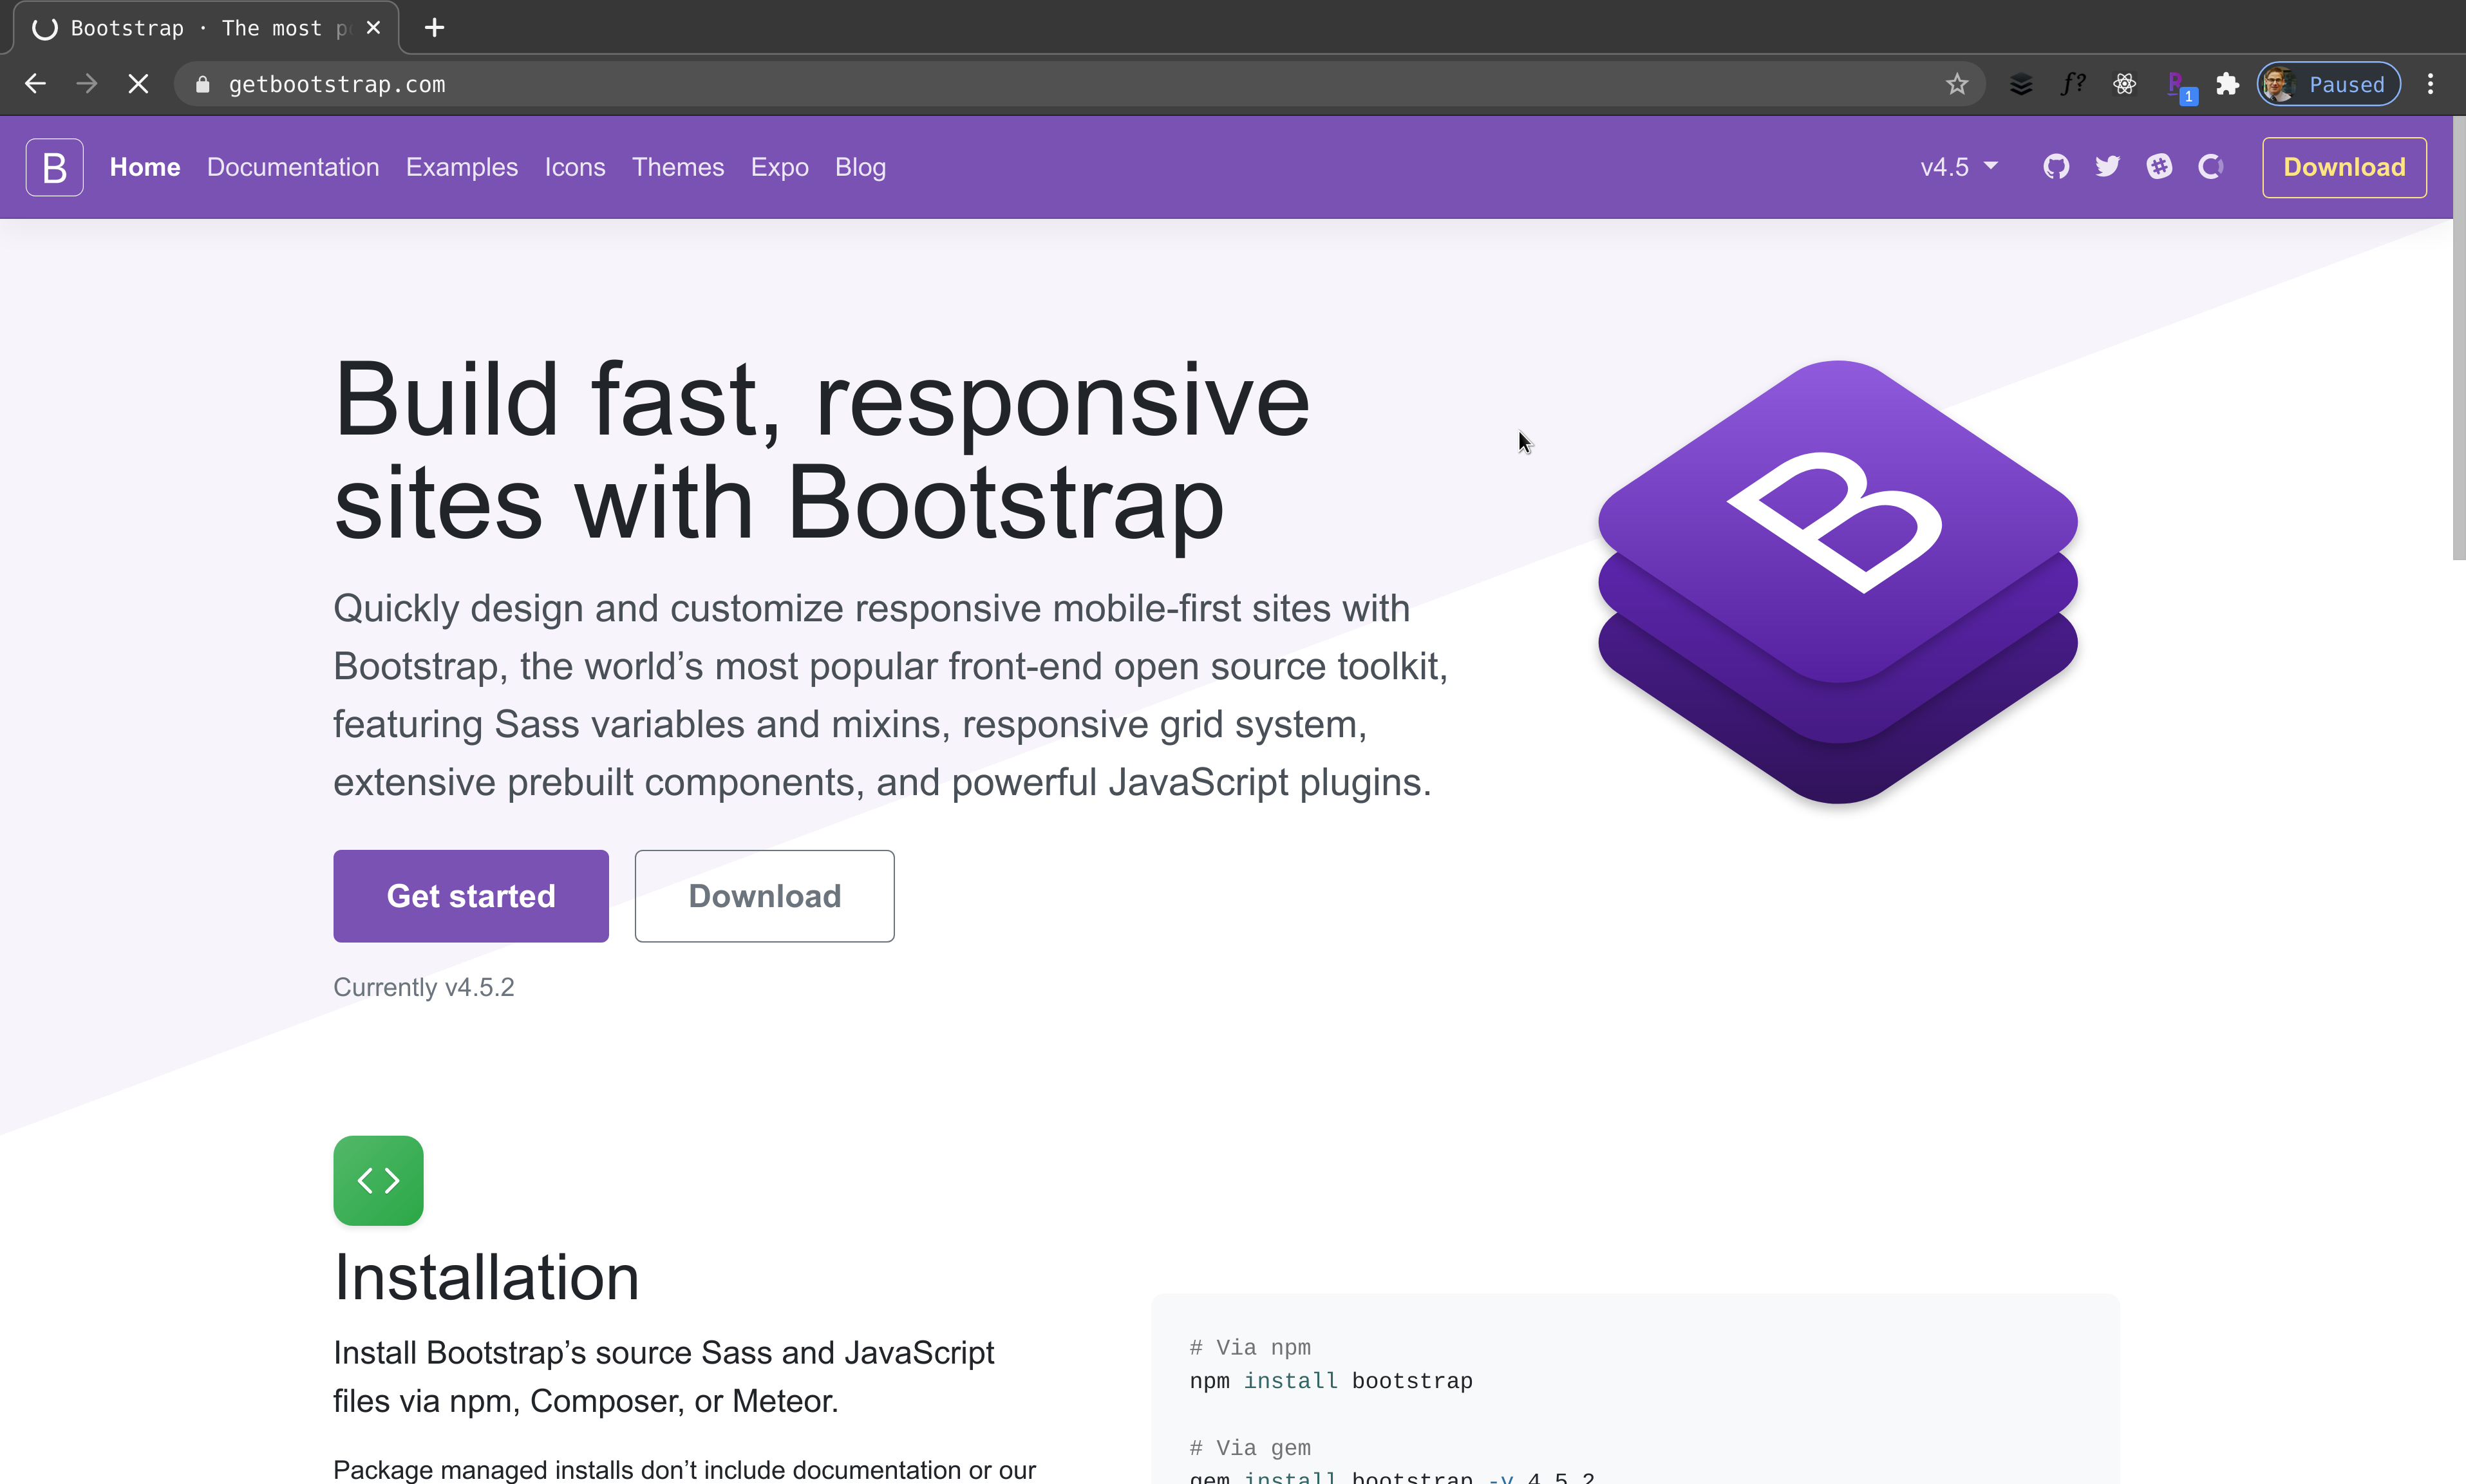
\includegraphics[scale=.085]{images/bootstrap-site.png}
    \caption{The figure's caption}
  \end{figure}
  %
\end{frame}

% Slide
%
\begin{frame}{Using CSS Grid for Responsive Web Design}
  %
  \begin{figure}
    \centering
    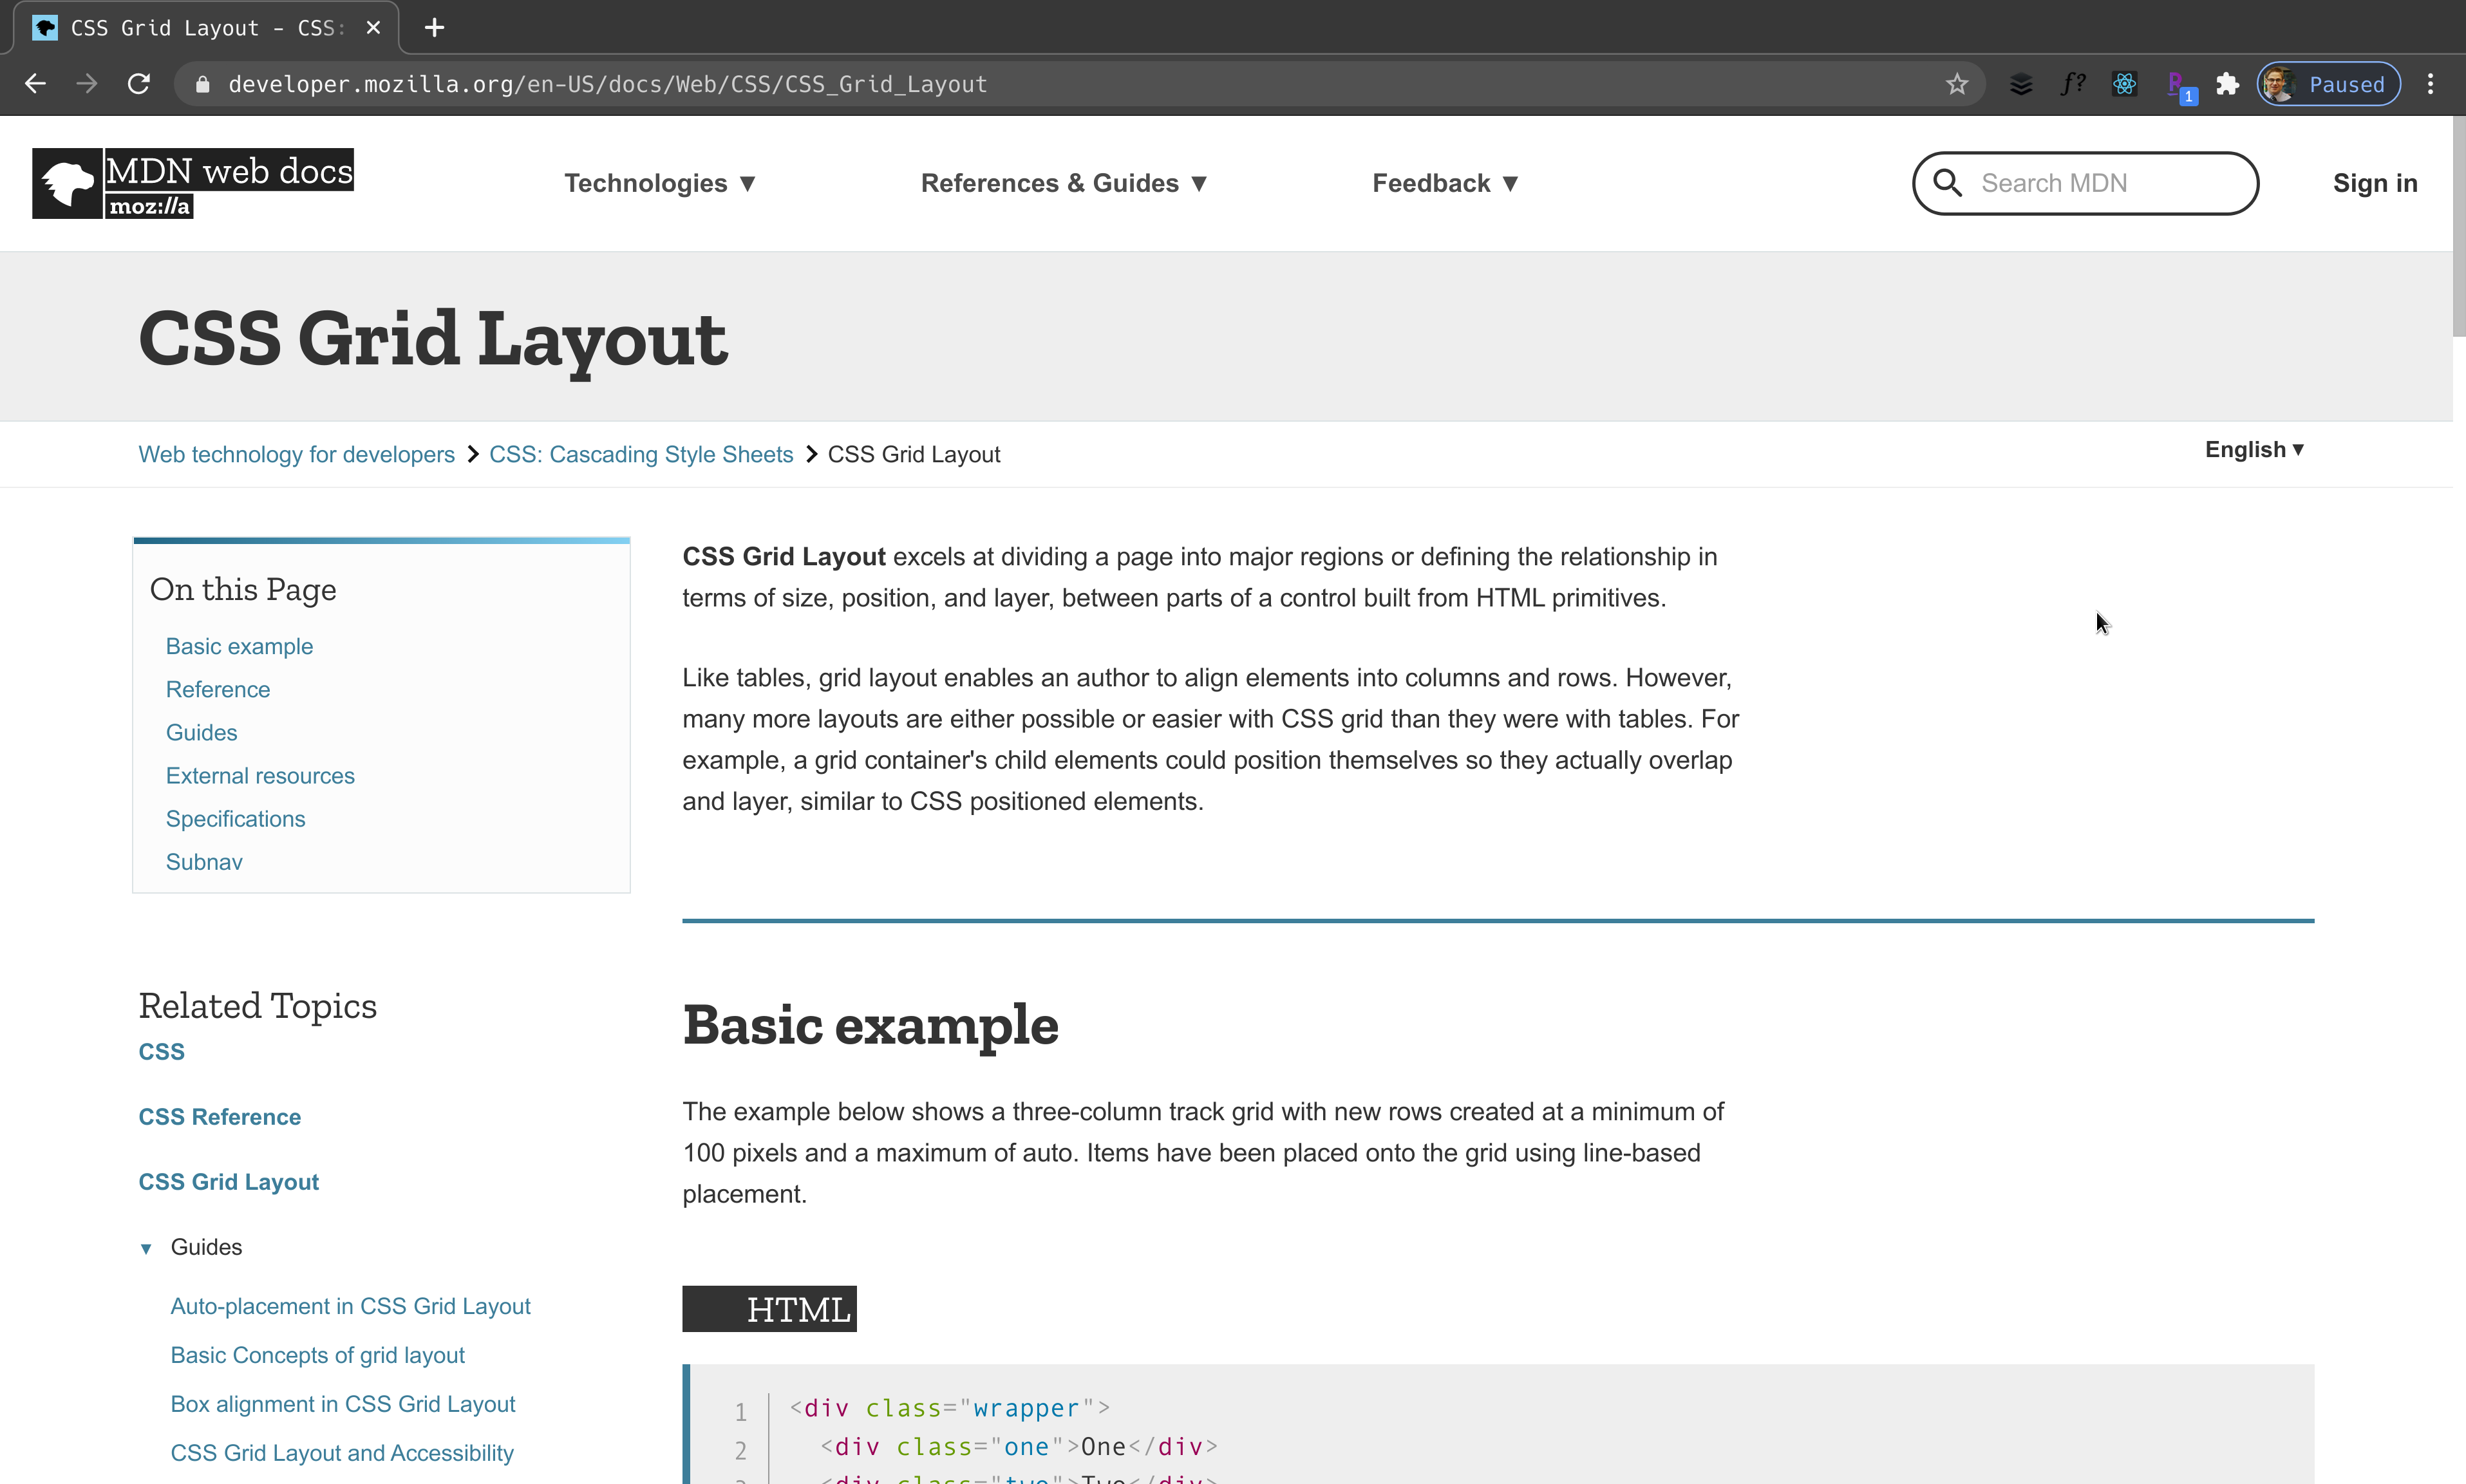
\includegraphics[scale=.085]{images/cssgrid-site.png}
    \caption{The figure's caption}
  \end{figure}
  %
\end{frame}

% Slide
%
\begin{frame}{Using Flexbox for Responsive Web Design}
  %
  \begin{figure}
    \centering
    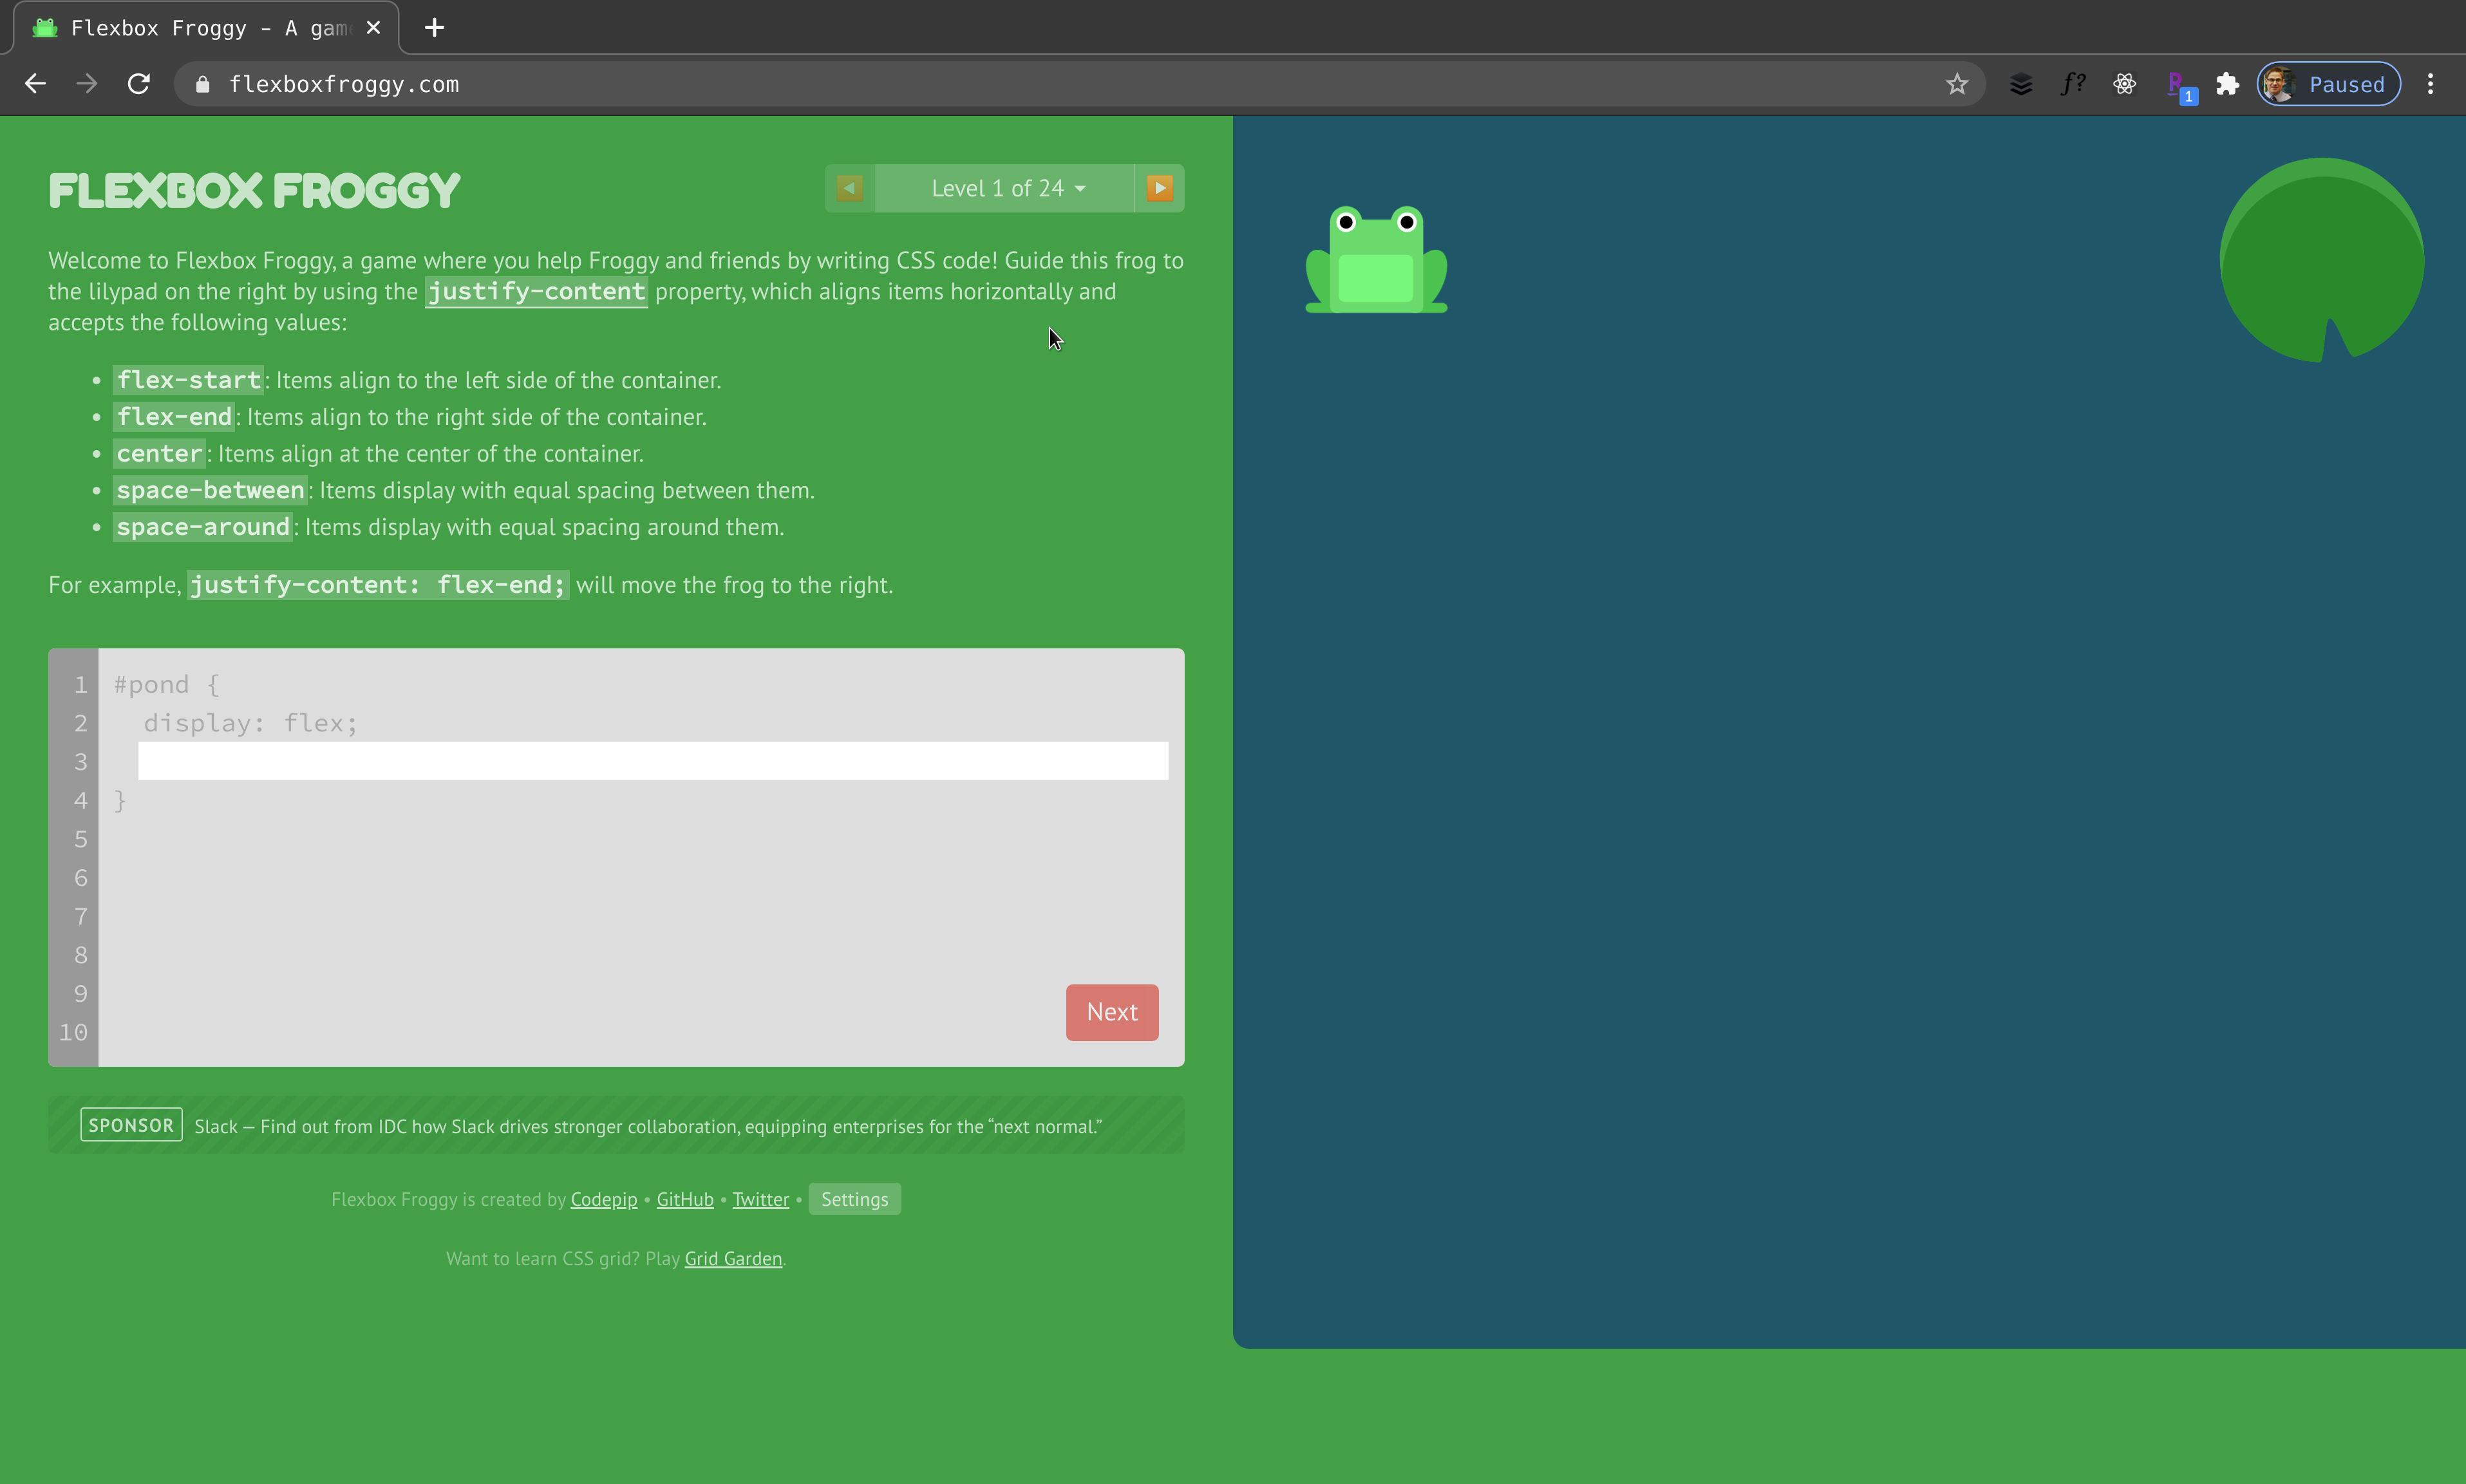
\includegraphics[scale=.085]{images/flexboxfroggy-site.png}
    \caption{The figure's caption}
  \end{figure}
  %
\end{frame}

\end{document}
